%!TEX root = ../main.tex

\chapter{Introduction}
\label{cha:introduction}

Unreachable Code Detection nowadays is integrated in almost every available static code analysis software as well as Integrated Development Environments and to some extent even compilers.
Unreachable Code is defined as Code that can never be reached, because either the program flow ended prematurely or due to unsatisfiable path conditions, as seen in Listing \ref{code:ex1}.
These types do not only increase the size of the program, but also increase the overall complexity of the source code or may even lead to unwanted behavior and errors (e.g., goto-fail bug \cite{Boyes_2014}).

\section{Motivation}
\label{sec:motivation}
Using Static code analysis to find errors before compiling, building or rolling out software is a very essential part of the software development process.
Static code analysis tools are able to identify a wide range of errors or make suggestions for adhering to a better style.
Finding errors in source code as it is written will not only make the program more robust, but also makes it more comprehensible, which leads to less time and energy needed during maintenance.
Especially unreachable, unnecessary and dead code are a main source of incomprehensible source code \cite{Romano_2020}.
In some instances unreachable code may be intended due to extensibility of the program \cite{Haas_2020} and may even not be clear if it is intended or not.
Before the breakthrough of the Object-Oriented Paradigm many Programs were developed in an imperative, procedural way. Some Styleguides of that time suggested splitting files into so many smaller files containing few functions or procedures \cite{Srivastava_1992}.
Interestingly, the emerge of the Object-Oriented Paradigm and its languages to the de facto standard increased the percentage of \emph{Unreachable - and Dead Code} \cite{Srivastava_1992}.
In extreme cases dead code may even lead to the so-called Anti-pattern Lava-Flow \cite{Romano_2020}, which typically occurs when Dead Code will not be removed and has to be maintained, even though it does not do much or even anything at all.
Systems that undergo constant evolution, like Web Systems, are also prone to lava-flow and Unreachable Code \cite{Boomsma_2012}.

\emph{Unreachable Code} is often confused with similar defects and different definitions are used.
It is often confused with dead code.

Analyzing these kinds if defects requires the program to be represented in form of a \emph{control flow graph} \ref{fig:cfg}.


\begin{program}[h!]
    \begin{GenericCode}
IF s_operationHour <> m_operationHour THEN
    m_operationHour := s_operationHour;
    IF s_operationHour = 0 THEN
        RESET_ALARM(Name := er_service, SubID1 := m_iNumber);
    END_IF;
    RETURN;
END_IF;
// s_operationHour must be equal to m_operationHour
IF s_operationHour = 0 THEN
    // unnecessary - already zero
    m_operationHour := 0;
    RESET_ALARM(Name := er_service, SubID1 := m_iNumber);
ELSE
    // unreachable
    IF s_operationHour <> m_operationHour THEN
        s_operationHour := m_operationHour;
    END_IF;
END_IF;\end{GenericCode}
    \caption{A minimal example containing unreachable code due to unsatisfiable conditions. The condition in line 15 is never reachable, since this case was already handeld in line 1 and the state of that variable did not change.}
    \label{code:ex1}
\end{program}
\begin{figure}[h!]
  \centering
  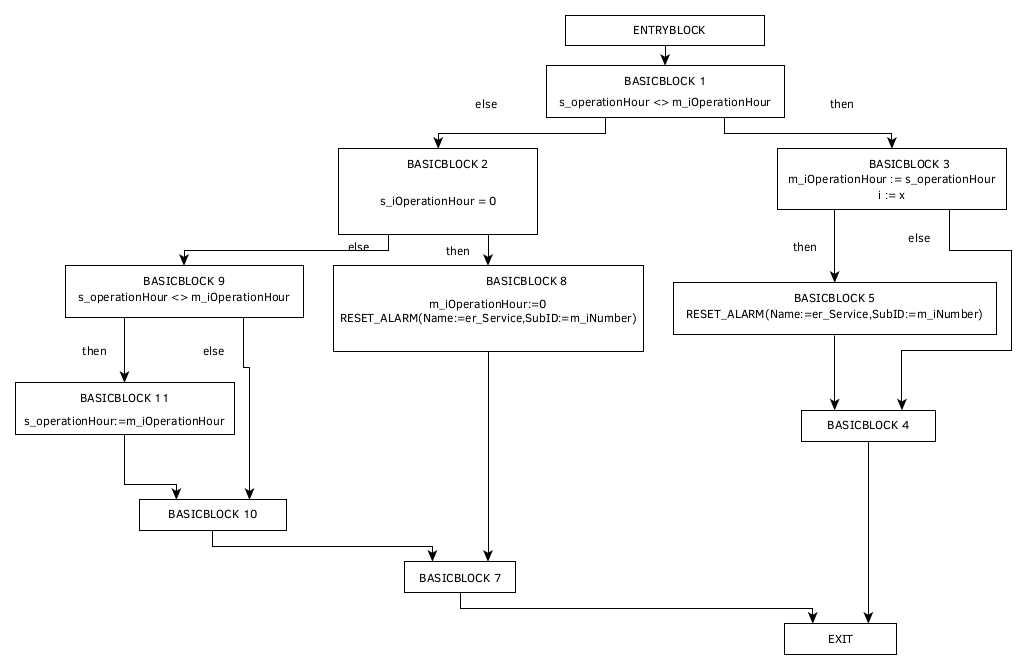
\includegraphics[width=1\textwidth]{minimal-example-cfg}
  \caption{The constructed control flow graph of Listing \ref{code:ex1}. Edges are marked either with then, describing the path if the condition results true, or else. Loops (and sometimes gotos) may easily be spotted since it is the only possibility for arrows pointing to former nodes.}
  \label{fig:cfg}
\end{figure}

It is worth mentioning that control flow graphs may be altered to make analysis easier, like single static assignment, which introduces many artificial variables to prevent redefinition of variables.

\section{Project Overview}
\label{sec:project overview}
This thesis is written as a part of a research project between the \emph{Software Competence Center Hagenberg GmbH} \cite{ScchGmbH} and \emph{Engel Austria GmbH} \cite{EngelGmbH}.
Engel produces injection molding machines, which are programmed using the \emph{Kemro-IEC} language, a dialect of the \emph{IEC 61131-3} standard language.
The project began as a joint work between the \emph{Software Competence Center Hagenberg} and the \emph{Johannes Kepler University Linz} \cite{jku, Prahofer_2012} within the competence centers program COMET of the Austrian Research Promotion Agency (FFG).
Over the years multiple rules identifying a wide range of errors were implemented, for example detecting unguarded division, where the divisor could potentially be zero, finding unused variables, highlighting high complexity of expressions, detecting dead code and other defects.
\clearpage
\pagebreak
\section{Objective of this thesis}
\label{sec:objective}
% Currently a rule for detecting unreachable Code is already in place, but is incomplete.
% The only kind of unreachable code that is detected when Statements stop the controlflow unconditionally (e.g. break, return, exit, goto, etc.).
% The goal is to identify as much unreachable code as possible correctly while minimizing the number of reported false positives.
% A popular approach to finding unreachable code is converting a controlflow graph into single static assignment form and using constant propagation \cite{Click_1995}.
% Afterwards conditions may be evaluated if they only consist of constants. The result (either true or false) determines if a given part of source code is always or never will be reachable (as mentioned before, only Conditions with constants only will be evaluated).
% This method is efficient and yields good results, but is not able to detect instance of unreachable code.
% \begin{program}
%    \begin{GenericCode}
% int $x_0$ $\leftarrow$ 1;
% do { $x_1$ $\leftarrow$ $\phi$($x_0$, $x_3$);
%     $b_0$ $\leftarrow$ ($x_{1}$ $\neq$ 1);
%     if( $b_0$ )
%         $x_2$ $\leftarrow$ 2;
%     $x_3$ $\leftarrow$ $\phi$($x_1$, $x_2$);
% } while ( pred() )
% return $x_3$;\end{GenericCode}
%    \caption{This Problem \cite{Click_1995} is the transformation to Single Static Assignment form, which does not check conditions and inserts a Phi-Function at line 6, even tough the condition in line 4 will never be satisfiable!}
%     \label{code:ssa-defect}
% \end{program}
% Finding these kind of Errors as seen in Listing \ref{code:ssa-defect} requires another approach, which does not rely on the transformation to single static assignment form.
% Part of this thesis is about using another method for unreachable code detection, which is able to find even more instances, while maintaining the same low reporting of false positives.
% The developed method will make usage of a satisfiable modulo theory prover (short: \emph{SMT-Solver}) and symbolic execution \cite{Arlt_2013}.


This thesis is structured into the following chapters:
\begin{itemize}
	\item \emph{Theoretical Foundation} defines the differences between unreachable, unnecessary and dead code will be defined. The standard IEC 61131-3 will also be presented, including provided languages and the structure of such programs. At last the concept of SMT solvers are explained and what use cases, they excel in.
	\item \emph{State of the Art} explores already existing tools targeting java source code. Beginning at the Java compiler itself to analyzers in integrated development environments to specialized plugins and services, which potentially could run in the cloud. It should be noted that all these described tools could be used together for maximum coverage.
	\item \emph{Finding unreachable code using a SMT-Solver} contains the idea and description of the implementation for discovering unreachable code. After an overview of the already existing architecture, the procedure of each step is described in detail.
	\item \emph{Evaluation} contains examples and their results/violations. These examples range from trivial to hard.
\end{itemize}
